% ============================================================
% Question Bank: ch09-01 What Is Probability?
% Topic Title: What Is Probability?
% CCSS: 7.SP.C.5
% Questions: 27 (15 MC + 6 SA + 6 Graphical)
% ============================================================

% --- Multiple Choice Questions (15) ---

\begin{practiceQuestion}{9-1-q01}{mc}
\begin{questionText}
Which value represents the probability of an event that is certain to happen?
\end{questionText}
\choiceA{$0$}
\choiceB{$\dfrac{1}{2}$}
\choiceC{$1$}
\choiceD{$2$}
\correctAnswer{C}
\explanation{A probability of $1$ means the event will definitely happen. Probability ranges from $0$ (impossible) to $1$ (certain), so $1$ represents certainty.}
\end{practiceQuestion}

\begin{practiceQuestion}{9-1-q02}{mc}
\begin{questionText}
A box contains $10$ tiles, each labeled with a different number from $1$ to $10$. What is the probability of drawing a tile labeled with a number greater than $10$?
\end{questionText}
\choiceA{$1$}
\choiceB{$\dfrac{1}{10}$}
\choiceC{$\dfrac{1}{2}$}
\choiceD{$0$}
\correctAnswer{D}
\explanation{There are no tiles labeled with a number greater than $10$, so this event is impossible. An impossible event has a probability of $0$.}
\end{practiceQuestion}

\begin{practiceQuestion}{9-1-q03}{mc}
\begin{questionText}
A teacher says the probability that the school library is open during school hours on a regular school day is $\dfrac{9}{10}$. Which best describes this event?
\end{questionText}
\choiceA{Impossible}
\choiceB{Unlikely}
\choiceC{Equally likely}
\choiceD{Very likely}
\correctAnswer{D}
\explanation{A probability of $\frac{9}{10} = 0.9$ is close to $1$. Probabilities near $1$ indicate the event is very likely to happen.}
\end{practiceQuestion}

\begin{practiceQuestion}{9-1-q04}{mc}
\begin{questionText}
Which of the following is NOT a valid probability for an event?
\end{questionText}
\choiceA{$0.45$}
\choiceB{$\dfrac{7}{8}$}
\choiceC{$1.2$}
\choiceD{$0$}
\correctAnswer{C}
\explanation{Probability must be a number between $0$ and $1$, inclusive. The value $1.2$ is greater than $1$, so it is not a valid probability.}
\end{practiceQuestion}

\begin{practiceQuestion}{9-1-q05}{mc}
\begin{questionText}
A jar contains $3$ red gumballs, $3$ blue gumballs, and $3$ yellow gumballs. If one gumball is chosen at random, what is the probability of choosing a yellow gumball?
\end{questionText}
\choiceA{$\dfrac{1}{9}$}
\choiceB{$\dfrac{1}{3}$}
\choiceC{$\dfrac{2}{3}$}
\choiceD{$\dfrac{3}{6}$}
\correctAnswer{B}
\explanation{There are $3$ yellow gumballs out of $3 + 3 + 3 = 9$ total. The probability is $\frac{3}{9} = \frac{1}{3}$.}
\end{practiceQuestion}

\begin{practiceQuestion}{9-1-q06}{mc}
\begin{questionText}
Sofia says the probability of picking a weekend day at random from the seven days of the week is about $0.29$. Which best describes this event?
\end{questionText}
\choiceA{Impossible}
\choiceB{Unlikely}
\choiceC{Equally likely as not}
\choiceD{Very likely}
\correctAnswer{B}
\explanation{There are $2$ weekend days out of $7$ total: $\frac{2}{7} \approx 0.29$. Since $0.29$ is closer to $0$ than to $\frac{1}{2}$, the event is unlikely but not impossible.}
\end{practiceQuestion}

\begin{practiceQuestion}{9-1-q07}{mc}
\begin{questionText}
A deck of cards has $4$ aces in $52$ cards. Which best describes the likelihood of drawing an ace at random?
\end{questionText}
\choiceA{Certain}
\choiceB{Very likely}
\choiceC{Equally likely as not}
\choiceD{Unlikely}
\correctAnswer{D}
\explanation{The probability is $\frac{4}{52} = \frac{1}{13} \approx 0.077$. Since this is close to $0$, drawing an ace is an unlikely event.}
\end{practiceQuestion}

\begin{practiceQuestion}{9-1-q08}{mc}
\begin{questionText}
A basketball player has made $48$ out of $50$ free throw attempts this season. Which probability best describes the chance that she makes her next free throw?
\end{questionText}
\choiceA{About $0$}
\choiceB{About $\dfrac{1}{2}$}
\choiceC{About $0.96$}
\choiceD{Exactly $1$}
\correctAnswer{C}
\explanation{She made $48$ out of $50$ attempts, so $\frac{48}{50} = 0.96$. This means making a free throw is very likely but not certain, since she has missed before.}
\end{practiceQuestion}

\begin{practiceQuestion}{9-1-q09}{mc}
\begin{questionText}
If the probability of an event is $\dfrac{1}{2}$, which statement best describes the event?
\end{questionText}
\choiceA{The event is impossible.}
\choiceB{The event will happen every time.}
\choiceC{The event is as likely to happen as not.}
\choiceD{The event is very unlikely.}
\correctAnswer{C}
\explanation{A probability of $\frac{1}{2}$ means the event has an equal chance of happening or not happening. This is called an even chance or equally likely event.}
\end{practiceQuestion}

\begin{practiceQuestion}{9-1-q10}{mc}
\begin{questionText}
A standard number cube with faces $1$ through $6$ is rolled. What is the probability of rolling a number less than $7$?
\end{questionText}
\choiceA{$0$}
\choiceB{$\dfrac{1}{6}$}
\choiceC{$\dfrac{6}{7}$}
\choiceD{$1$}
\correctAnswer{D}
\explanation{Every face on a standard number cube ($1, 2, 3, 4, 5, 6$) is less than $7$. Since every outcome is favorable, the probability is $\frac{6}{6} = 1$, making this a certain event.}
\end{practiceQuestion}

\begin{practiceQuestion}{9-1-q11}{mc}
\begin{questionText}
At a veterinary office, records show that $7$ out of $10$ appointments are for dogs. What is the probability that the next appointment is NOT for a dog?
\end{questionText}
\choiceA{$\dfrac{7}{10}$}
\choiceB{$\dfrac{3}{7}$}
\choiceC{$\dfrac{3}{10}$}
\choiceD{$\dfrac{10}{7}$}
\correctAnswer{C}
\explanation{The probability of a dog appointment is $\frac{7}{10}$. The probability of NOT a dog is $1 - \frac{7}{10} = \frac{3}{10}$.}
\end{practiceQuestion}

\begin{practiceQuestion}{9-1-q12}{mc}
\begin{questionText}
Which of these events has a probability closest to $\dfrac{1}{2}$?
\end{questionText}
\choiceA{Rolling a $6$ on a standard number cube}
\choiceB{Drawing a vowel from the letters of the word ORANGE}
\choiceC{Landing on tails when tossing a fair coin}
\choiceD{Picking a red card from a bag of $1$ red and $9$ blue cards}
\correctAnswer{C}
\explanation{A fair coin has exactly $2$ equally likely outcomes, so the probability of tails is $\frac{1}{2}$. This is the closest to $\frac{1}{2}$ among all the options.}
\end{practiceQuestion}

\begin{practiceQuestion}{9-1-q13}{mc}
\begin{questionText}
A traffic light is green for $30$ seconds, yellow for $5$ seconds, and red for $25$ seconds per cycle. What is the probability that the light is green when a car arrives at a random time?
\end{questionText}
\choiceA{$\dfrac{1}{4}$}
\choiceB{$\dfrac{1}{3}$}
\choiceC{$\dfrac{1}{2}$}
\choiceD{$\dfrac{5}{12}$}
\correctAnswer{C}
\explanation{The total cycle time is $30 + 5 + 25 = 60$ seconds. The light is green for $30$ seconds, so the probability is $\frac{30}{60} = \frac{1}{2}$.}
\end{practiceQuestion}

\begin{practiceQuestion}{9-1-q14}{mc}
\begin{questionText}
If the probability that it will snow tomorrow is $0.15$, what is the probability that it will NOT snow?
\end{questionText}
\choiceA{$0.15$}
\choiceB{$0.50$}
\choiceC{$0.85$}
\choiceD{$1.15$}
\correctAnswer{C}
\explanation{The probability of an event and its complement sum to $1$. So $P(\text{not snow}) = 1 - 0.15 = 0.85$.}
\end{practiceQuestion}

\begin{practiceQuestion}{9-1-q15}{mc}
\begin{questionText}
A bag contains only blue and green beads. The probability of drawing a green bead is $\dfrac{5}{8}$. Which statement is true?
\end{questionText}
\choiceA{The probability of drawing a blue bead is $\dfrac{5}{8}$.}
\choiceB{It is more likely to draw a blue bead than a green bead.}
\choiceC{It is more likely to draw a green bead than a blue bead.}
\choiceD{Drawing a blue bead is impossible.}
\correctAnswer{C}
\explanation{The probability of green is $\frac{5}{8}$ and blue is $1 - \frac{5}{8} = \frac{3}{8}$. Since $\frac{5}{8} > \frac{3}{8}$, green is more likely.}
\end{practiceQuestion}

% --- Short Answer Questions (6) ---

\begin{practiceQuestion}{9-1-q16}{sa}
\begin{questionText}
A bag contains $6$ red, $4$ white, and $2$ black marbles. What is the probability of NOT drawing a red marble? Express your answer as a simplified fraction.
\end{questionText}
\correctAnswer{$\frac{1}{2}$}
\explanation{There are $4 + 2 = 6$ non-red marbles out of $6 + 4 + 2 = 12$ total. The probability is $\frac{6}{12} = \frac{1}{2}$.}
\end{practiceQuestion}

\begin{practiceQuestion}{9-1-q17}{sa}
\begin{questionText}
The probability that a train arrives on time is $0.92$. What is the probability that the train does NOT arrive on time?
\end{questionText}
\correctAnswer{$0.08$}
\explanation{Complementary events sum to $1$. The probability of not arriving on time is $1 - 0.92 = 0.08$.}
\end{practiceQuestion}

\begin{practiceQuestion}{9-1-q18}{sa}
\begin{questionText}
A standard number cube is rolled. List the probability that the result is a prime number. Express your answer as a simplified fraction.
\end{questionText}
\correctAnswer{$\frac{1}{2}$}
\explanation{The prime numbers on a standard cube are $2, 3, 5$ — that is $3$ favorable outcomes out of $6$ total. So $\frac{3}{6} = \frac{1}{2}$.}
\end{practiceQuestion}

\begin{practiceQuestion}{9-1-q19}{sa}
\begin{questionText}
A month is chosen at random from the $12$ months of the year. What is the probability that it starts with the letter J? Express your answer as a simplified fraction.
\end{questionText}
\correctAnswer{$\frac{1}{4}$}
\explanation{The months starting with J are January, June, and July — that is $3$ out of $12$ months. The probability is $\frac{3}{12} = \frac{1}{4}$.}
\end{practiceQuestion}

\begin{practiceQuestion}{9-1-q20}{sa}
\begin{questionText}
An event has a probability of $\dfrac{3}{5}$. Is this event more likely to happen or not happen?
\end{questionText}
\correctAnswer{More likely to happen}
\explanation{Since $\frac{3}{5} = 0.6 > 0.5$, the event is more likely to happen than not. A probability greater than $\frac{1}{2}$ means the event is more likely to occur.}
\end{practiceQuestion}

\begin{practiceQuestion}{9-1-q21}{sa}
\begin{questionText}
A box contains letter tiles for the word MATHEMATICS. If one tile is chosen at random, what is the probability of choosing a letter that is NOT a vowel? Express your answer as a simplified fraction.
\end{questionText}
\correctAnswer{$\frac{7}{11}$}
\explanation{MATHEMATICS has $11$ letters: M, A, T, H, E, M, A, T, I, C, S. The vowels are A, E, A, I ($4$ letters), so consonants are $11 - 4 = 7$. The probability of choosing a consonant is $\frac{7}{11}$.}
\end{practiceQuestion}

% --- Graphical Multiple Choice Questions (3) ---

\begin{practiceQuestion}{9-1-q22}{gmc}
\begin{questionText}
A probability scale is shown below. At which position should the event ``flipping heads on a fair coin'' be placed?

\begin{center}
\begin{tikzpicture}
  \draw[thick,->] (0,0) -- (10.5,0);
  \foreach \x/\lab in {0/0, 2.5/0.25, 5/0.50, 7.5/0.75, 10/1.00} {
    \draw[thick] (\x,0.15) -- (\x,-0.15) node[below]{\lab};
  }
  \node[above] at (0,0.3) {Impossible};
  \node[above] at (5,0.3) {Even chance};
  \node[above] at (10,0.3) {Certain};
  \node[above,funRed] at (1.25,0.7) {\textbf{W}};
  \node[above,funBlue] at (5,0.7) {\textbf{X}};
  \node[above,funGreen!70!black] at (7.5,0.7) {\textbf{Y}};
  \node[above,funOrange] at (10,0.7) {\textbf{Z}};
\end{tikzpicture}
\end{center}
\end{questionText}
\choiceA{Position W}
\choiceB{Position X}
\choiceC{Position Y}
\choiceD{Position Z}
\correctAnswer{B}
\explanation{Flipping heads on a fair coin has a probability of $\frac{1}{2} = 0.50$, which is an even chance. Position X is at $0.50$ on the scale.}
\end{practiceQuestion}

\begin{practiceQuestion}{9-1-q23}{gmc}
\begin{questionText}
Look at the probability line below. Four events are placed on it.

\begin{center}
\begin{tikzpicture}
  \draw[thick] (0,0) -- (12,0);
  \draw[thick] (0,0.15) -- (0,-0.15) node[below]{$0$};
  \draw[thick] (6,0.15) -- (6,-0.15) node[below]{$0.5$};
  \draw[thick] (12,0.15) -- (12,-0.15) node[below]{$1$};
  \filldraw[funRed] (0.6,0) circle (4pt) node[above=6pt]{\footnotesize Event P};
  \filldraw[funBlue] (5.4,0) circle (4pt) node[above=6pt]{\footnotesize Event Q};
  \filldraw[funGreen!70!black] (8.4,0) circle (4pt) node[above=6pt]{\footnotesize Event R};
  \filldraw[funOrange] (11.4,0) circle (4pt) node[above=6pt]{\footnotesize Event S};
\end{tikzpicture}
\end{center}

Which event is most likely to happen?
\end{questionText}
\choiceA{Event P}
\choiceB{Event Q}
\choiceC{Event R}
\choiceD{Event S}
\correctAnswer{D}
\explanation{On a probability line, events closer to $1$ are more likely. Event S is positioned closest to $1$, so it is the most likely to occur.}
\end{practiceQuestion}

\begin{practiceQuestion}{9-1-q24}{gmc}
\begin{questionText}
The bar graph below shows how many of each color bead are in a bag.

\begin{center}
\begin{tikzpicture}
  \begin{axis}[
    ybar, bar width=20pt, ymin=0, ymax=12,
    ylabel={Number of Beads},
    symbolic x coords={Red, Blue, Green, White},
    xtick=data,
    nodes near coords,
    width=8cm, height=6cm,
    enlarge x limits=0.25
  ]
  \addplot[fill=funRed!70] coordinates {(Red,8) (Blue,4) (Green,6) (White,2)};
  \end{axis}
\end{tikzpicture}
\end{center}

If one bead is chosen at random, which color is the most likely to be chosen?
\end{questionText}
\choiceA{Red}
\choiceB{Blue}
\choiceC{Green}
\choiceD{White}
\correctAnswer{A}
\explanation{Red has the most beads ($8$ out of $8 + 4 + 6 + 2 = 20$). A higher count means a higher probability: $\frac{8}{20} = \frac{2}{5}$, which is the greatest among the four colors.}
\end{practiceQuestion}

% --- Graphical Short Answer Questions (3) ---

\begin{practiceQuestion}{9-1-q25}{gsa}
\begin{questionText}
The table below shows the contents of a prize bag at a school carnival.

\begin{center}
\begin{tabular}{|l|c|}
\hline
\textbf{Prize} & \textbf{Number in Bag} \\
\hline
Pencil & $12$ \\
\hline
Eraser & $8$ \\
\hline
Sticker & $5$ \\
\hline
Bookmark & $5$ \\
\hline
\end{tabular}
\end{center}

What is the probability of randomly drawing a sticker or a bookmark? Express your answer as a simplified fraction.
\end{questionText}
\correctAnswer{$\frac{1}{3}$}
\explanation{There are $5 + 5 = 10$ stickers and bookmarks combined out of $12 + 8 + 5 + 5 = 30$ total prizes. The probability is $\frac{10}{30} = \frac{1}{3}$.}
\end{practiceQuestion}

\begin{practiceQuestion}{9-1-q26}{gsa}
\begin{questionText}
Look at the probability number line below.

\begin{center}
\begin{tikzpicture}
  \draw[thick,->] (0,0) -- (10.5,0);
  \foreach \x/\lab in {0/0, 2/0.2, 4/0.4, 6/0.6, 8/0.8, 10/1.0} {
    \draw[thick] (\x,0.15) -- (\x,-0.15) node[below]{\lab};
  }
  \filldraw[funBlue] (7,0) circle (4pt) node[above=6pt]{Event A};
\end{tikzpicture}
\end{center}

Event A is placed at approximately $0.7$ on the probability line. What is the probability that Event A does NOT happen?
\end{questionText}
\correctAnswer{$0.3$}
\explanation{Complementary events sum to $1$. If $P(\text{Event A}) \approx 0.7$, then $P(\text{not Event A}) = 1 - 0.7 = 0.3$.}
\end{practiceQuestion}

\begin{practiceQuestion}{9-1-q27}{gsa}
\begin{questionText}
A vending machine has the following snacks loaded equally across its $20$ slots:

\begin{center}
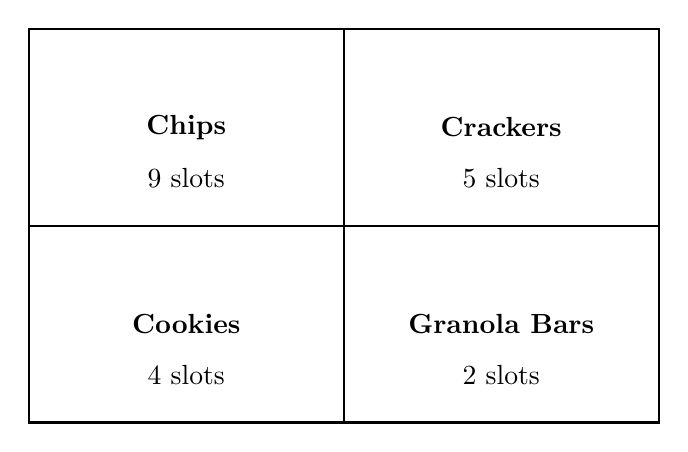
\begin{tikzpicture}
  \draw[thick] (0,0) rectangle (8,5);
  \draw[thick] (0,2.5) -- (8,2.5);
  \draw[thick] (4,0) -- (4,5);
  \node at (2,3.75) {\textbf{Chips}};
  \node at (2,3.1) {$9$ slots};
  \node at (6,3.75) {\textbf{Crackers}};
  \node at (6,3.1) {$5$ slots};
  \node at (2,1.25) {\textbf{Cookies}};
  \node at (2,0.6) {$4$ slots};
  \node at (6,1.25) {\textbf{Granola Bars}};
  \node at (6,0.6) {$2$ slots};
\end{tikzpicture}
\end{center}

If a snack is dispensed at random, what is the probability that it is NOT chips? Express your answer as a simplified fraction.
\end{questionText}
\correctAnswer{$\frac{11}{20}$}
\explanation{There are $9$ chip slots out of $20$ total, so $P(\text{chips}) = \frac{9}{20}$. The probability of NOT chips is $1 - \frac{9}{20} = \frac{11}{20}$.}
\end{practiceQuestion}
